\chapter{Analysis}

\section{Artificial Intelligence} % Alternative AI Models and Prompt Engineering
- AI
- machine learning
- deep learning (neural networks)

\subsection{AI Models}
Describe:
Text-to-image, text-to-text, text-to-audio

LLMs - Large Language Models (use neural networks)
GPTs - Generative Pre-Trained Transformers

\subsection{Prompt engineering}
Describe what is

\section{Risks of implementing AI solutions}

\subsection{Ethical risks}
Content generation based on copyrighted material (Copyrighted material as input)
people compromising 
compromising and harmful media 
deep fakes
etc.

\subsection{Moral risks}
Sexual / Violent content (bombs, weapons), forbidden language (illegal activities)
Military use
etc.

\subsection{Security risks}
social engineering
Malware generation and recursive training of malware samples
Targeted phishing - voice clone, video/image generation of targeted person
etc.

\section{Content filters}
Why are they, and what purpose do they serve

\subsection{Jailbreak}
jailbreak patching = cat and mouse game
    one side develops new jailbreak
    other patches it and the cycle repeats itself
experimenting with jailbreaks
yoda jailbreak try (bing - does not work, maybe try better prompt)
experimenting with content filters (hardcoded, others, etc)

\section{Methods of Attacks}



\section{Legislation}

\subsection{EU AI Act}





% TAKTO SA ROBI FIGURE/OBRAZOK

% Figure \ref{fig:dynabook}:

% \begin{figure}[h]
% \begin{centering}
% 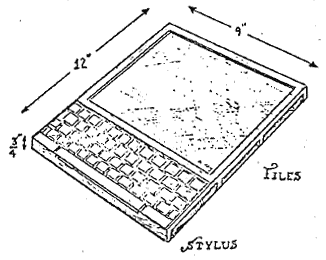
\includegraphics[width=5cm]{assets/images/Dynabook}
% \par\end{centering}
% \caption{Dynabook \label{fig:dynabook}}
% \end{figure}